\documentclass{article}
\usepackage{parskip}
\usepackage{listings}
\usepackage{pdfpages}
\usepackage[margin=.6in]{geometry}
\begin{document}
\includepdf[pages=5]{Module5}
Comes from greek for secret writing. Cryptography is just making a plaintext message secret. Cryptography is a part of Cryptology which also includes cryptoanalysis which is when we try to do the reverse.
	
\includepdf[pages=7]{Module5}
We standardize our fictional characters. 
\begin{itemize}
	\item Alice, Bob, Carol, Dave - good honest hacker
	\item Eve - a passive eavesdropper that can't do anything
	\item Mallory - man in the middle
	\item Trent - trusted third party
\end{itemize}

\includepdf[pages=8]{Module5}
Confidentiality means we want to prevent Even from reading Alice's messages. We can do this using a cryptosystem

Integrity says we want to prevent Mallory from modifying Alice's messages. We can do this through message authentication (MACs), signature schemes, or cryptographic hash functions (not very secure since hackers can do this easily).

Privacy says we want to prevent MAllory from impersonating Alice. We can do this by passwords or biometrics and such, or through challenge response protocols.

A secret-key system or a public-key system. With a public key system we have two keys. A public key that anyone can use to encrypt something, and a secret private key that can be used to decrypt stuff. A secret key system can be block (requiring data to be a fixed width) or stream.


\includepdf[pages=9]{Module5}
We should only ever rely on a simple secret key that is easy to change. We could have a bunch of different encryption functions. This is not always practical so we encrypt with a long key that varies each time. A system is only as secure as the possible number of keys (we want the widest variety of keys to prevent brute forcing). Even then it is always possible to brute force no matter how long your key is. 

\includepdf[pages=10]{Module5}
A \textbf{strong crypto system} is one where iterating through every possible key is the best possible attack. 

\includepdf[pages=11]{Module5}
Frequently the attacker can get a small bit of plaintext from cypher text. For instance HTTP headers tend to be fairly standard so intercepting an encrypted request allows you to figure out a little bit. Breaking the enigma machine was done by getting a bunch of plaintext cyphertext pairs and analyzing them for a bit before breaking the code. To get these plain/cypher pairs they listened to this one base in russia that would send the same message every day (``weather report: all clear''). 



































\end{document}